\documentclass[11pt]{article}

% Packages
\usepackage{amsmath}
\usepackage{graphicx}
\usepackage{lipsum}
\usepackage{fancyhdr}
\usepackage{tabularx}
\usepackage{caption}
\usepackage{hyperref}
\usepackage{float}

\renewcommand{\headrulewidth}{0pt}
\renewcommand{\footrulewidth}{0pt}

% Document
\begin{document}

\begin{titlepage} % Title page environment
\centering % Center all text
\vspace*{1cm} % Adjust the vertical space as needed

\includegraphics[width=0.5\textwidth]{../images/logo.png}\\[1cm] % Include your company logo and adjust size
{\Huge\bfseries Product Asssessment}\\[0.5cm] % Main title in a large bold font
{\Large for Alpha Corp}\\[0.2cm] % Subtitle in a slightly smaller font
{\Large June 2024}\\[2cm] % Date
{\Large Version 1.0}\\[1cm] % Version number
\vfill % Fill the vertical space
{\large Prepared by John Doe}\\[2cm] % Author
{\small PentestPros }\\ % Company details
{\small https://pentest.pros}\\ % Company website
{\small mailto:hello@pentest.pros}\\ % Company email
\end{titlepage}

\pagestyle{fancy}
\lhead{}
\chead{Client Confidential}
\rhead{}
\lfoot{}
\cfoot{\thepage}
\rfoot{}

\tableofcontents

\pagebreak

\section{Executive Summary}

\lipsum[1]

\lipsum[2]

\lipsum[4]

\lipsum[3]

\subsection{Immediate Next Steps}

The following immediate next steps are recommended to address the critical security findings identified during the assessment:

\begin{itemize}
    \item \lipsum[9][1]
    \item \lipsum[9][2]
    \item \lipsum[9][3]
\end{itemize}

\pagebreak

\section{Strategic Recommendations}

\lipsum[10][1-8]

\lipsum[14][1-8]

\lipsum[14][1-6]

\lipsum[13][1-6]

\lipsum[12][1-5]

\lipsum[11][1-5]

\lipsum[15][1-3]

\lipsum[16][1-2]

\lipsum[16][3-4]

\pagebreak

\section{Document Control}

\subsection{Assessment Metadata}

The following table describes from of the key information for this assessment.

\begin{table}[h]
\centering
\begin{tabular}{|l|l|}
\hline
\textbf{Assessment Title} &  Product Assessment \\ \hline
\textbf{Report ID} & AC-001-01 \\ \hline
\textbf{Proposal Reference} & AC-01 \\ \hline
\textbf{Client Representative} & Bob Anders \\ \hline
\textbf{Engagement Manager} & John Doe \\ \hline
\textbf{Date} & June 2024 \\ \hline
\textbf{Classification} & Client Confidential \\ \hline
\end{tabular}
\caption{Assessment Metadata}
\end{table}

\subsection{Version History}

The following table describes the document control information for this assessment.

\begin{table}[h]
\centering
\begin{tabular}{|l|l|l|l|}
\hline
\textbf{Version} & \textbf{Date} & \textbf{Author} & \textbf{Change Summary} \\ \hline
0.1 & 2024-06-01 & John Doe & Initial Draft \\ \hline
0.2 & 2024-06-02 & Jane Doe & Initial Review \\ \hline
1.0 & 2024-06-04 & John Doe & Released to client \\ \hline
\end{tabular}
\caption{Document Control}
\end{table}


\lipsum[123]

\pagebreak

\subsection{Report Distribution}

The following table describes the distribution of this report.

\lipsum[124]

\begin{table}[h]
\centering
\begin{tabular}{|l|l|l|}
\hline
\textbf{Organisation} & \textbf{Name} & \textbf{Job Title} \\ \hline
Example Consulting Ltd & John Doe & Security Consultant \\ \hline
Alpha Corp & Bob Anders & CISO \\ \hline
Alpha Corp & Chris Smith & IT Manager \\ \hline
\end{tabular}
\caption{Report Distribution}
\end{table}

\newpage

\subsubsection{Warranty Notice}

\lipsum[125]
\vspace{6pt}
\lipsum[125]

\pagebreak

\section{Assessment Overview}

\subsection{Scope}

\lipsum[66]

\lipsum[67]

\subsection{Caveats}

\lipsum[68][2]

\lipsum[68][2]

\lipsum[69][1]

\subsection{Findings Overview}

The following table provides an overview of the assessment findings by risk rating:

\begin{table}[h]
\centering
\begin{tabular}{|l|l|}
\hline
\textbf{Risk Rating} & \textbf{Findings} \\ \hline
High & 1 \\ \hline
\end{tabular}
\caption{Findings Overview}
\end{table}

The assessment identified a total of 8 findings across different risk ratings. The findings will be detailed in the following sections.

\newpage

\subsection{List of Findings}

The assessment findings are categorized based on the phase of the assessment and the risk rating of the findings. The findings are presented in the following sections:

\subsubsection{External Infrastructure}

\begin{table}[ht]
\centering % This centers the table that follows
\begin{tabularx}{\textwidth}{|l|l|l|X|}
\hline
\textbf{Rating} & \textbf{ID} & \textbf{Title} \\ \hline
High & AC-1-1 & Jenkins Server Exposed to the Internet \\ \hline
\end{tabularx}
\end{table}
\captionof{table}{List of Findings} % Providing a caption for the table, using captionof from the caption package

\pagebreak

\section{Assessment Findings}

\subsection{Phase 1: External Infrastructure}

\phantomsection % Create a hyperreference point here
\addcontentsline{toc}{subsubsection}{ Jenkins Server Exposed to the Internet} % Add custom entry to the ToC

\begin{table}[h!]
    \noindent
    \begin{tabularx}{\linewidth}{lX}
        \textbf{AC-1-1} & \textbf{ Jenkins Server Exposed to the Internet}
    \end{tabularx}
    \begin{tabularx}{\linewidth}{XXX}
        Risk: High  & Likelihood: High & Impact: High \\
    \end{tabularx}
\end{table}

\textbf{Description}

\lipsum[1][1-5]
\vspace{6pt}
\lipsum[2][6]:

\begin{figure}[H]
    \centering
    \setlength{\fboxrule}{1pt} % Sets the thickness of the border
    \setlength{\fboxsep}{5pt}  % Sets the padding between the border and the image
    \fbox{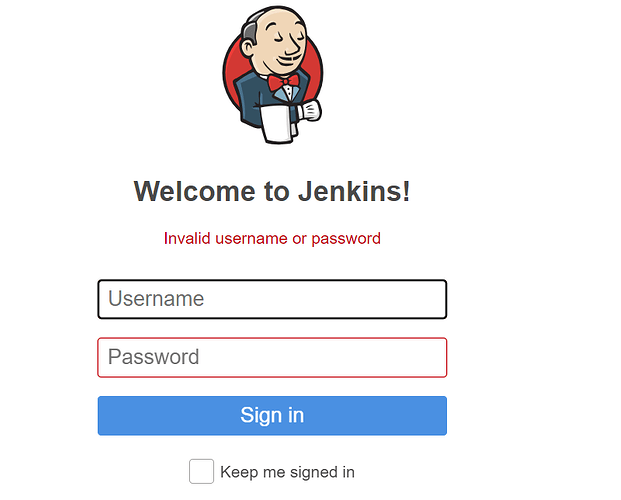
\includegraphics[width=0.8\textwidth]{../images/img.png}}
    \caption{Jenkins Server Configuration}
\end{figure}

\lipsum[2][1-5]

\newpage

\textbf{Recommendation}

\lipsum[9]
\vspace{6pt}
\lipsum[6][1-2]
\vspace{6pt}
\lipsum[7][1-3]\footnote[1]{http://docs.jenkins.com \label{jenkins-server}}

\textbf{Location}

\begin{itemize}
    \item \lipsum[8][1]
    \item \lipsum[8][2]
    \item \lipsum[8][3]
\end{itemize}

\newpage

\section{Appendix}
This section contains supplemental data from assessment findings, additional assessment metadata, or other information that may otherwise clutter the main body of this report.

\subsection{Assessment Team}

The following individuals were involved in the assessment:

\begin{table}[h]
\centering
\begin{tabular}{|l|l|l|l|}
\hline
\textbf{Name} & \textbf{Role} & \textbf{Job Title} & \textbf{Notes} \\
John Doe & Team Lead & Security Consultant & OSCP \\ \hline
Jane Doe & Team Member & Security Consultant & CISSP \\ \hline
\end{tabular}
\caption{Team Information}
\end{table}

\newpage

\subsection{Risk Rating Definitions}

The following risk rating definitions were used during the assessment:

\begin{table}[ht]
    \centering
    \begin{tabularx}{\textwidth}{|c|X|}
        \hline
        \textbf{Risk Rating} & \textbf{Definition} \\
        \hline
        \textbf{Critical} & A vulnerability that could be exploited by an attacker to gain unauthorized access to critical systems or data. \\
        \hline
        \textbf{High} & A vulnerability that could be exploited by an attacker to gain unauthorized access to sensitive systems or data. \\
        \hline
        \textbf{Medium} & A vulnerability that could be exploited by an attacker to gain unauthorized access to non-sensitive systems or data. \\
        \hline
        \textbf{Low} & A vulnerability that has a limited impact on the security of the system or data. \\
        \hline
        \textbf{Informational} & A finding that represents no security risk but may be useful to document. \\
        \hline
    \end{tabularx}
    \caption{Risk Rating Definitions}
\end{table}

\end{document}